\title{Reconstruction of strange attractors via inter-spike intervals}
\author{\`Alex Arcas Cuerda \& Ram\'on Marc Garcia Seuma}
\date{\today}
\documentclass[10pt]{article}

\usepackage[a4paper, total={7in, 10in}]{geometry}
\usepackage{graphicx}
\usepackage{amsmath}

\begin{document}
\maketitle
\section{Introduction}

\section{Geometry from a Time Series}

\subsection{Summary}

The idea of \cite{paper1} is to give some insight in turbulent or chaotic systems. To do so, they enfatice that the usual data in this experiments is some observable of the system sampled at regular times. 

First, they show the fact that one can reconstruct the topology of such a systems just with one coordinate of any dynamical system. Really, what they show is that one can reconstruct the topology of the system using any combination of $D$ independent variables of the systems, where $d$ is the dimension of the system. They show that this procedure works for the Rossler attractor.

Then, they show that for a systems with only one positive-characteristic exponent(Liapunov exponent in modern terms), one can extract it just using the description defined above ergo one only needs one coordinate to find the exponent. They compute these exponents with different descriptions for the Rossler attractor. and show how well the results fit with the exponent extracted from the 3-coordinate one.

Finally, they state that one can obtain the dimensionality of an attractor from using the description used above. To do so they give a 'general' procedure in which one graphs the conditional probability of a coordinate being a certain value knowing $k$ previous values. Then, they state that the $k$ for which the graph displays a kind of delta, or a peak as sharp as possible, is the dimension of the attractor. They use that to extract that the dimension of the Rossler attractor is two.

\subsection{Review}

We first find this paper really interesting and in fact we still do. Despite, we have some major objections to it, to start with they don't really \textit{prove} anything they just show that they've found it works that way and they give some examples to support it's hypothesis. Being more precise, they don't show why the topology of the phase space is conserved using their logic so it can all be wrong. In fact, Takens theorems \cite{takens} proves what they conjecture but arguing why the fit is not the dimension of the dynamical system but two times. Moreover, the procedure they give to compute the dimension of the attractor it's latter proved to be effective only in really \textit{flat} strange attractors and for the Rossler case it isn't exactly two.

So our final review would sum up that they found some really important intuition about dynamical systems given some \textit{time series} of it but they had much work to do yet. We have to remember that the paper is from 1979 and at that time the knowledge of strange attractors was really short.

\section{Reconstruction of Dynamical Systems from Interspike Intervals}

\subsection{Summary}
The paper \cite{interspike} tries to pose the following question: being a point process a the manifestation of an an underlying deterministic system, it is possible to identify the states of the system from the information provided in those sequence of points? The point process is simply a series of event timings. The main motivation of this question comes from examples found typically in biology, particularly in microbiological systems, where amplitude measurements of an observable, such as neuronal currents, are not possible (nor desirable), but a series of pulses or spikes emitted at certain times are recorded. In the case of the neurons, for example, we normally have the firing times, emitted when the cell reaches a threshold potential, which triggers depolarization and then the cycle is restarted.\\
On the other hand, they rely on the fact that states of finite dimensional dynamical systems correspond in a one-to-one manner with delay-coordinate vectors, which are vectors of time series measurements of a generic system observable. System analysis of this type is suggested in and an embedding theorem due to Takens established its validity. This has great consequences and applications, because we can analyse topology and even geometry of the chaotic attractor. The applications can be noise filtering, prediction of chaotic time series.\\
Takens' theorem \cite{takens}. It is a delay embedding theorem, i.e it gives the conditions under which a chaotic dynamical system can be reconstructed from a sequence of observations of the state of the system. The important point is that the reconstruction preserves the properties of the system that do not change under smooth coordinate changes. Nonetheless, it does not preserve the geometric shape of structures in phase space. The theorem basically states that the strange attractor can be embedded in $k-$ dimensional Euclidean space with $k>2d_A$, being $d_A$ the box counting dimension $d_A$.\\
Thus the paper, relying the Takens' theorem, analyse the previous question for inter-spike interval (ISI) data, assuming a generic integrate-and-fire model coupling deterministic dynamical systems to a spike train, so that there is assumed that there is a one-to-one correspondence between the states of the system and the inter-spike interval vectors of sufficiently large dimension. \\
Thus they create signals $S(x)$, being $x$ the trajectories provided by the dynamical system described by the Rossler and Lorentz attractors. Then the firing times $T_i$ are inferred recursively by the equation
\begin{equation}
\int_{T_i}^{T_{i+1}} S(t)dt=\Theta
\end{equation}
And from this, the inter-spike intervals are defined as $t_i = T_i - T_{i-1}$. Those intervals can define the ISI vectors $(t_i,...,t_{i-m+1})$, m took in accordance to the Takens's theorem, so that it can be used to reconstruct the attractor $X$. Using different types of signal for the different analysis they perform, they reconstruct a Rossler attractor, but they later focus on the Lorentz dynamics. In order to determine that deterministically driven ISI series can be distinguished from stochastically driven ISI series, they perform a prediction algorithm in the inter-spike intervals obtained from the deterministic system and to some series of what is called surrogate data. They show that there is predictability not explained by any of the null hypotheses controlled for by the surrogate data. As the threshold $\Theta$ increases, predictability of the series decreases. They also analyse the effect of lengthening the prediction horizon, showing that there is several-step-ahead predictability in the original ISI series.

\subsection{Review}
There are several points that seems to have a lack of purpose or explanation in the paper. They seem to take specific signals, apparently arbitrary, although they specify it is obviously needed positive signals in order to have spike events. They just reconstruct the Rossler attractor (they also write wrong the equations of this dynamical system), and give no explanation on why the Lorentz one its not observable from the spike interval time. They also fix the embedding dimension $m=3$, giving little explanation So we had the feeling that most of the calculations and parameters are taken to confirm the results; although they claim at the beginning of the paper that their goal is to develop a model which is as generic as possible, their choices are not well justified, and there are some points that can not be fully understood by simply following the paper even the references. Nevertheless, it shows interesting results that seem to have important implications and we were able to reproduce its most important results with the parameters given by them.

\section{Results}
Now we present all the results we reproduced from the papers reviewed above. We basically analyse the Rossler and Lorentz systems.\\
First, we reconstruct a finite-dimensional phase-space picture of the sampled system's time evolution, corresponding to the Rossler equations.

\begin{center}
\includegraphics[scale=0.5]{rossler_xprima}
\caption{Reconstruction $(x,\dot x)$ from the time series for the Rossler attractor}
\label{fig:rossler_xprima}
\end{center}

Then we focus on the interspike intervals. First of all, we create trajectories of the Rossler dynamics. Using this trajectories, we put the signal $S(x)=x(t)+40$ and threshold $\Theta=20$, so we obtain the ISI time series, and then the can define the interspike intervals.

\begin{center}
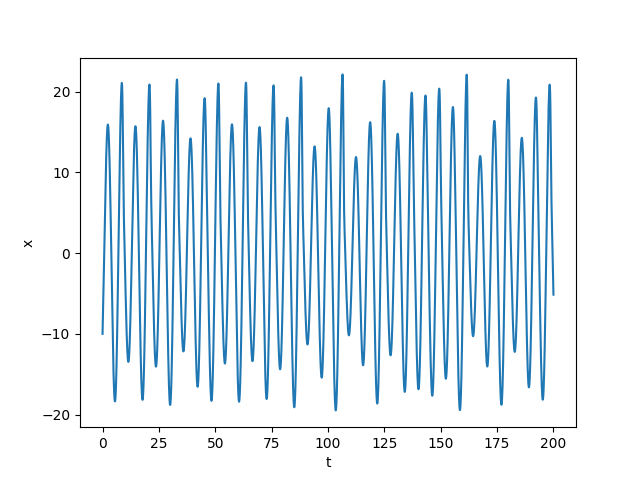
\includegraphics[scale=0.5]{real_trajectory_rossler} 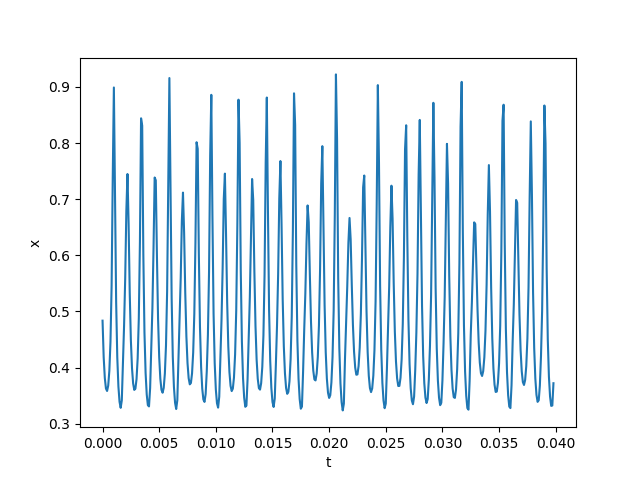
\includegraphics[scale=0.5]{reconstructed_trajectory_rossler}
\caption{Deterministic trajectory from equations described above (left) for the Rossler system and an ISI series generated from this.}
\label{fig:rossler_xprima}
\end{center}

Then we can create the vectors $(t_i,t_{i+1},t_{i+2})$. This allows us to reconstruct again the phase portrait for the Rossler attractor by connecting vectors.

\begin{center}
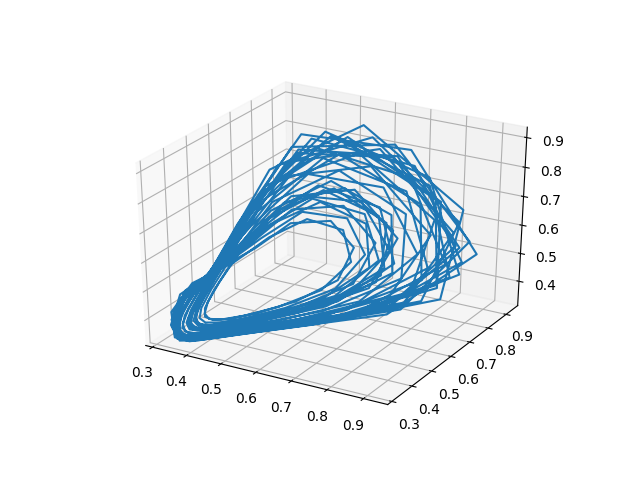
\includegraphics[scale=0.5]{rossler_atractor_400points}
\caption{Reconstructed phase portrait for the Rossler attractor using ISI's with $400$ points.}
\label{fig:rossler_isi}
\end{center}

We can do the same analysis for the Lorentz equations. Although the geometry in the phase portrait is not conserved, here the form of the attractor obtained is not particularly interesting. Nevertheless, the analysis are still valid and we proceed to use the information stored in the ISI series to unveil the topollogy of the dynamical system.

\begin{center}
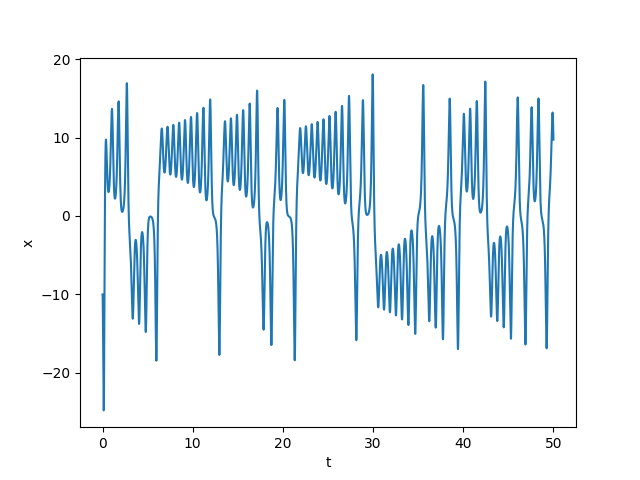
\includegraphics[scale=0.5]{real_trajectory_lorentz}
\caption{Deterministic trajectory from equations described above for the Lorentz system.}
\label{fig:lorentz_trajectory}
\end{center}

We use the signal $S(t)=(x(t)+2)^2$ and different thresholds to do the analysis of the prediction error algorithm described in the section of the paper \cite{interspike}. So we basically apply the nonlinear prediction algorithm to interspike intervals for the Lorentz system. Then we create surrogate data \cite{surrogate}, specifically we use the Gaussian-scaled shuffle (GS) surrogate, which is a random shufHe of the original series subject to retaining much of the serial correlation. The GS surrogate corresponds to the null hypothesis that the series is a monotonically scaled version of amplitudes produced by a Gaussian random process. We fix the embedding dimension $m=3$ and predicted one step ahead $(h=1)$, for increasing thresholds $\Theta$, in order to see that the predictability of the series decrease, and tends to disappear as the threshold is big enough.

\begin{center}
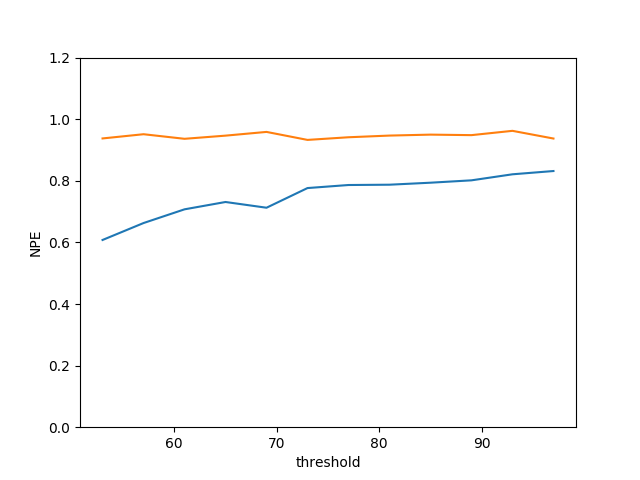
\includegraphics[scale=0.5]{NPE_12series}
\caption{Normalized one step ahead prediction error for several ISI series with varying $\Theta$, for the original ISI series and the GS surrogate.}
\label{fig:12series}
\end{center}

We also show the comparison for the ISI lenght density distribution obtained on this cases for both series (original and surrogate)

\begin{center}
%\includegraphics[scale=0.5]{ISIdistribution} \includegraphics[scale=0.5]{GSdistribution}
\caption{.}
\label{fig:distributions}
\end{center}

\section{Conclusions}

\begin{thebibliography}{99}
 
\bibitem{prove}N. H. Packard, J. P. Crutchfield, J. D. Farmer, and R. S. Shaw, {\it Geometry from a Time Series}, Dynamical Systems Collective, Physics DePartment, University of California, Santa Crae, California (13 November 1979).

\bibitem{interspike}Tim Sauer, {\it Reconstruction of Dynamical Systems from Interspike Intervals}, Department of Mathematical Sciences, Geode Mason University, Fairfas, Vinpnia (Received 15 February 1994).

\bibitem{takens}F. Tskens, {\it Dynamical Systems and Turbulence}, Lecture Notes in Math-
ematics Vol. 898 (Springer-Verlsg, Berlin, 1981).

\end{thebibliography}

\end{document}